
%
%  $Description: Author guidelines and sample document in LaTeX 2.09$ 
%
%  $Author: ienne $
%  $Date: 1995/09/15 15:20:59 $
%  $Revision: 1.4 $
%

\documentclass[times, 10pt,twocolumn]{article} 
\usepackage{paper}
\usepackage{times}
\usepackage{graphicx}
\usepackage{float}
\usepackage{amsmath}

%\documentstyle[times,art10,twocolumn,latex8]{article}

%------------------------------------------------------------------------- 
% take the % away on next line to produce the final camera-ready version 
% \pagestyle{empty}

%------------------------------------------------------------------------- 
\begin{document}

\title{18-752 Final Project Report: EMG Signal Classification}

\author{Paul Griffioen\\Dept. of Electrical and Computer Engineering\\Carnegie Mellon University\\ pgriffi1@andrew.cmu.edu\\
% For a paper whose authors are all at the same institution, 
% omit the following lines up until the closing ``}''.
% Additional authors and addresses can be added with ``\and'', 
% just like the second author.
\and
Thomas Mayo-Smith\\Dept. of Electrical and Computer Engineering\\Carnegie Mellon University\\tmayosmi@andrew.cmu.edu\\
}

\maketitle
\thispagestyle{empty}

%------------------------------------------------------------------------- 
\begin{abstract}
The main objective of this project was to improve upon the existing method of EMG signal classification 
used by a software package called CAPS by improving classification accuracy and classification latency.
To achieve this objective we explored the ability of a gaussian mixture model (GMM) to preform blind identification 
and detection on a novel data set collected using CAPS. Using the labels generated by the GMM we then explored the
ability of an exponential likelihood with a categorical prior for supervised identification and detection.
Both methods very clearly appear to classify EMG samples more accurately than CAPS, but it appeared
that only the GMM was fully capable of reducing classification latency.
\end{abstract}

%------------------------------------------------------------------------- 
\section{Introduction and Motivation}
It has been widely reported that prosthesis patients abandon advanced prosthetic limbs capable of being controlled
via EMG signals as a result of having too much difficulty learning how to isolate their muscle contractions in 
a way which a prosthetic limb can understand them. To alleviate this frustration special games
controlled via EMG signals have been developed to make pre-prosthetic training more effective. Unfortunately
the method used by the existing software package which classifies EMG signals during game play is inaccurate 
and irritating to use. In this work we explore the ability of a GMM and an exponential distribution with a
categorical prior to classify EMG signals as game actions. In particular the game we experiment with is Space
Invaders$^{\tiny{\textregistered}}$ and EMG signals produced when a player is flexing, extending, co-contracting and
resting his/her forearm are classified as "move left", "move right", "shoot" and "do nothing" respectively. Our
results show that the proposed methods of EMG signal classification are advantageous to use over the existing one
as a result of their lower classification latency and better ability to cluster different types of EMG signals.

%------------------------------------------------------------------------- 
\section{Data Set Collection}
Using a custom sleeve lined with eight EMG electrodes which sampled at 100Hz and the software package
CAPS for data collection we recorded two games of Space Invaders$^{\tiny{\textregistered}}$ (Figure 1). Each EMG sample 
consisted of a vector of 9 values the first of which corresponded to the classification label determined by the
CAPS software and the next 8 of which corresponded to the absolute values of the electrograms read from
the 8 EMG electrodes at a particular point during the game. CAPS only uses sample values from channels
1 and 4 to make a classification because when most people put on the custom sleeve these channels are
on opposite sides of the forearm muscle and are thus best suited to distinguish between the muscle contractions
a player performs during Space Invaders$^{\tiny{\textregistered}}$ game play. By observing histograms of sample values from each
channel it was clear channels other than 4 and 1 corresponded to muscles not used very much during gameplay (Figure 2).
The histograms of these other channels in many cases tended to be similar across contractions and noisy. 
CAPS claimed in its documentation to make classifications using a simple threshold method; however, this was
was not clearly observed in the data we collected likely due to noise and imprecise hardware measurements
(Figure 3). As a result we reclassified the data using by manually implementing the threshold method (Figure 4).
Limits of this classification method are clearly illustrated in (Figure 5). 

%------------------------------------------------------------------------- 
\section{Blind Identification and Detection}
Our first strategy to improve EMG signal classification was to use a GMM for blind Identification and detection.
The GMM was composed of four bivariate gaussians each of which was had parameters with a categorical distribution.
Each gaussian was intended to fit the EMG data corresponding to each contraction and the dimensions of each
gaussian corresponded to the two channels being used for classification. The categorical prior corresponded the
likelihood of a particular contraction during game play. Equations 1 - 5 summarize this GMM model.

\begin{equation}
x = \text{EMG sample}
\end{equation}
\begin{equation}
\lambda_i = \text{contraction }i, i\in[1,2,3,4]
\end{equation}
\begin{equation}
f_{\mu_i,\sigma_i^2}(x|\lambda_i) = \mathcal{N}(\mu_i,\sigma_i^2)
\end{equation}
\begin{equation}
f_{\mathbf{p}}(\lambda) = \text{categorical density with parameters } p_i
\end{equation}
\begin{equation}
f(x) = \sum_{i=1}^{4}f_{p}(\lambda_i)f_{\mu_i,\sigma_i^2}(x|\lambda_i)
\end{equation}

The MLE of the parameters of the GMM can be solved via equations 6 - 9.

\begin{equation}
L(\mu,\sigma^2, p, \lambda, X) = \log{f_{\mu,\sigma^2,p}(X)} = \sum_{k=1}^{n}\log{\sum_{i=1}^{4}f_{\mu_i,\sigma_i^2}(x_k|\lambda_i)f_{p}(\lambda_i)}
\end{equation}
\begin{equation}
\frac{\partial}{\partial{\mu}}L(\mu,\sigma^2,p, \lambda,X) = 0 \text{ } => \text{ } \hat{\mu}
\end{equation}
\begin{equation}
\frac{\partial}{\partial{\sigma^2}}L(\mu,\sigma^2,p,\lambda,X) = 0 \text{ } => \text{ } \hat{\sigma}^2
\end{equation}
\begin{equation}
\frac{\partial}{\partial{p}}L(\mu,\sigma^2,p,\lambda,X) = 0 \text{ } => \text{ } \hat{p}
\end{equation}

There is no closed form solution for the MLE of the parameters of the GMM and solving numerically via
Newtons method or gradient decent is slow so we decided to use the Expectation Maximization algorithm. Parameters
of the GMM are initialized using the data which was poorly labeled by the threshold method. For instance,
the initial mean of the gaussian which we expected to eventually fit flexion samples was initialized to mean of the
data points labeled flexion by the threshold method. Initializing parameters this way eliminated the need to take
additional steps to figure out which gaussian corresponded to a particular contraction type after the GMM parameters
had converged. Equations 10 - 13 summarize the EM algorithm we used. \\

E-Step

\begin{equation}
f_{\theta_i}(\lambda_i|x) = \frac{f_{\theta_i}(\lambda_i)\prod_{\text{channel}}f_{\theta_i}(x|\lambda_i)}{\sum_{i=1}^{4}f_{\theta_i}(\lambda_i)\prod_{\text{channel}}f_{\theta_i}(x|\lambda_i)}
\end{equation}

M-Step

\begin{equation}
f_{\mu_i,\sigma_i^2}(\lambda_i|x) = \frac{1}{n}\sum_{k=1}^{n}f_{\hat{\mu}_i,\hat{\sigma}_i^2}(\lambda_i|x_k)
\end{equation}
\begin{equation}
\mu_i = \frac{\sum_{k=1}^{n}f_{\hat{\mu}_i,\hat{\sigma}_i^2}(\lambda_i|x_k)x_k}{\sum_{k=1}^{n}f_{\hat{\mu}_i,\hat{\sigma}_i^2}(\lambda_i|x_k)}
\end{equation}
\begin{equation}
\sigma_i^2 = \frac{\sum_{k=1}^{n}f_{\hat{\mu}_i,\hat{\sigma}_i^2}(\lambda_i|x_k)(x_k-\mu_i)(x_k-\mu_i)^T}{\sum_{k=1}^{n}f_{\hat{\mu}_i,\hat{\sigma}_i^2}(\lambda_i|x_k)}
\end{equation}

The EM algorithm is set to stop iterating after either a maximum number of 1000 iterations or if the maximum update to a particular parameter is less that .01.
Once the parameters of the GMM have been estimated detection is done via equation 14.

\begin{equation}
\hat{\lambda} = \max_{i}f_{\theta_i}(\lambda_i|x)
\end{equation}

Results for this method can be seen in Figures 6, 7 and 8.


%------------------------------------------------------------------------- 
\section{Supervised Identification and Detection}

Supervised Identification and Detection.
\begin{equation}
x = \text{EMG sample}
\end{equation}
\begin{equation}
\lambda_i = \text{contraction }i, i\in[1,2,3,4]
\end{equation}
\begin{equation}
f_{\theta_i}(x|\lambda_i) = \theta_i\mathrm{e}^{-\theta_ix}
\end{equation}
\begin{equation}
f_{\theta_i}(\lambda_i) = (\text{\# data points for }\lambda_i)/(\text{total \# of labeled data points})
\end{equation}


\begin{equation}
L(\theta_i,\lambda_i,X) = \log{f_{\theta_i}(X|\lambda_i)} = \log{\prod_{k=1}^{n}f_{\theta_i}(x_k|\lambda_i)} = \sum_{k=1}^{n}\log{f_{\theta_i}(x_k|\lambda_i)}
\end{equation}
\begin{equation}
\frac{\partial}{\partial{\theta_i}}L(\theta_i,\lambda_i,X) = 0 \text{ } => \text{ } \hat{\theta}_i = \frac{n}{\sum_{k=1}^{n}x_k}
\end{equation}
\begin{equation}
f_{\theta_i}(\lambda_i|x) = \frac{f_{\theta_i}(\lambda_i)\prod_{\text{channel}}f_{\theta_i}(x|\lambda_i)}{\sum_{i=1}^{4}f_{\theta_i}(\lambda_i)\prod_{\text{channel}}f_{\theta_i}(x|\lambda_i)}
\end{equation}
\begin{equation}
\hat{\lambda} = \max_{i}f_{\theta_i}(\lambda_i|x)
\end{equation}



%------------------------------------------------------------------------- 
\nocite{ex1,ex2}
\bibliographystyle{paper}
\bibliography{paper}

%\begin{thebibliography}{}
\begin{thebibliography}{}\setlength{\itemsep}{-1ex}\small

\bibitem{incentives}
Author. "Title." \textit{Journal}, pp. \#-\#, Year.

\end{thebibliography}

\section{Appendices}
\begin{figure}
  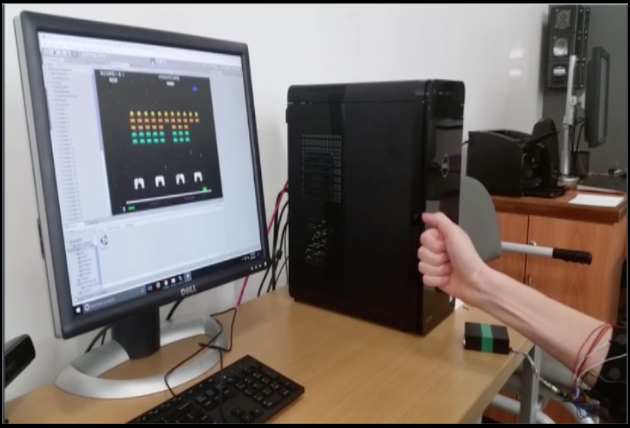
\includegraphics[width=\linewidth]{Figures/f1.png}
  \caption{Data Collection}
  \label{fig:data_collection}
\end{figure}

\begin{figure}
  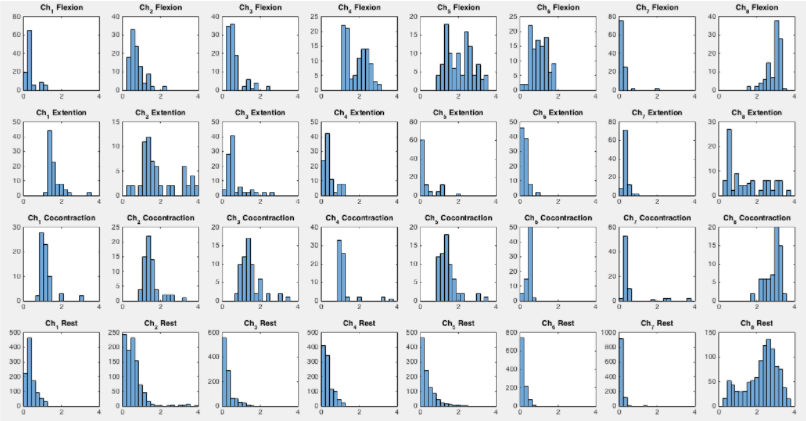
\includegraphics[width=\linewidth]{Figures/f2.png}
  \caption{Each histogram$_{i,j}$ shows the distribution of EMG samples for contraction$_i$ and channel$_j$.}
  \label{fig:histogram}
\end{figure}

\begin{figure}
  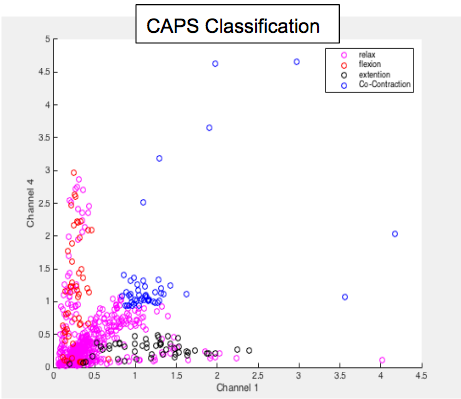
\includegraphics[width=\linewidth]{Figures/f3.png}
  \caption{Contraction clusters determined by the CAPS software. CAPS only uses electrogram values from Ch 1 and Ch 4 for classification.}
  \label{fig:caps_clusters}
\end{figure}

\begin{figure}
  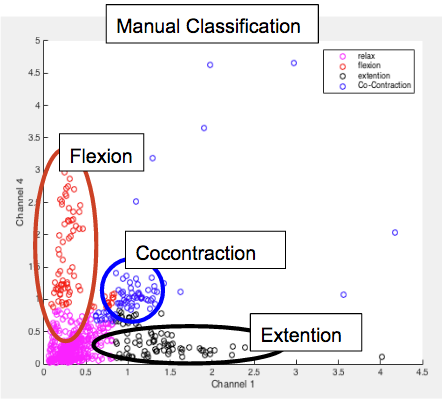
\includegraphics[width=\linewidth]{Figures/f4.png}
  \caption{Contraction clusters determined by the manually implemented CAPS algorithm.}
  \label{fig:manual_clusters}
\end{figure}

\begin{figure}
  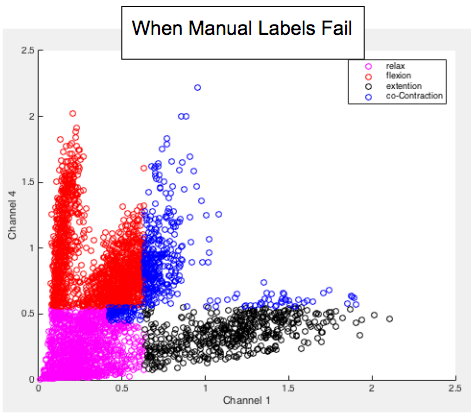
\includegraphics[width=\linewidth]{Figures/f5.png}
  \caption{Linear decision boundaries of CAPS algorithm are not appropriate for classification.}
  \label{fig:manual_clusters_fail}
\end{figure}

\begin{figure}
  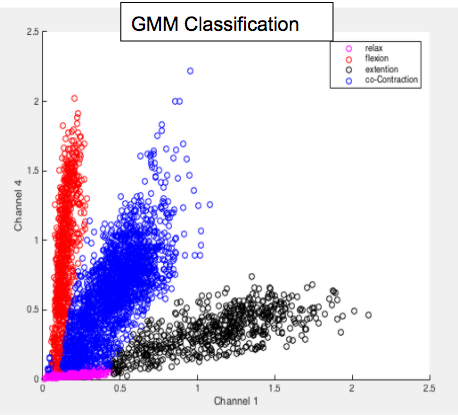
\includegraphics[width=\linewidth]{Figures/f6.png}
  \caption{Contraction clusters determined by GMM.}
  \label{fig:gmm_clusters}
\end{figure}

\begin{figure}
  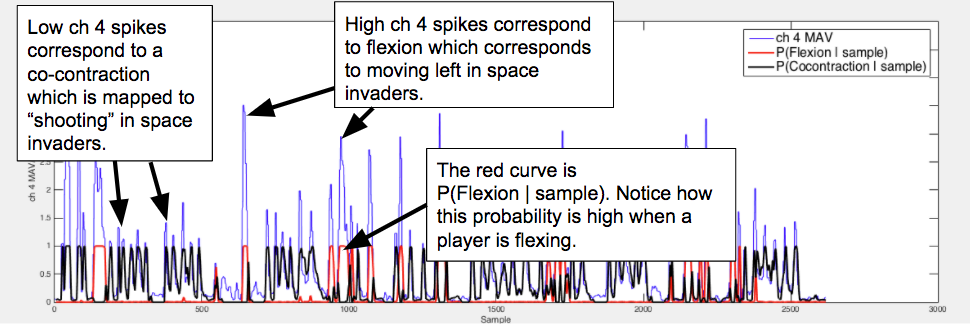
\includegraphics[width=\linewidth]{Figures/f7.png}
  \caption{Posterior probabilities of flexion and co-contraction overlaid on top Ch 4 EMG signal.}
  \label{fig:posterior_probabilities}
\end{figure}

\begin{figure}
  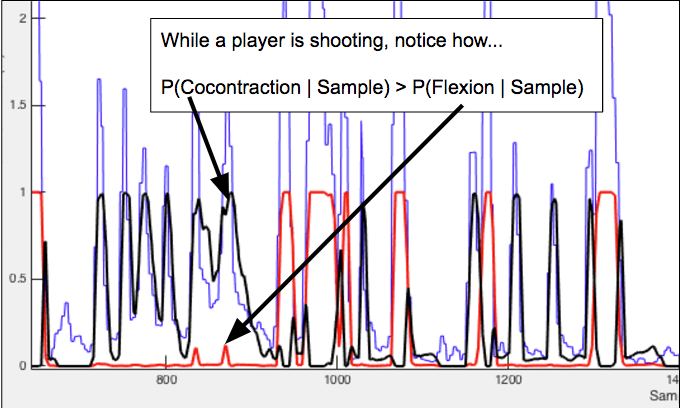
\includegraphics[width=\linewidth]{Figures/f8.png}
  \caption{Close up of Figure 7.}
  \label{fig:posterior_probabilities_close_up}
\end{figure}

\end{document}
